\documentclass[a4paper,lithuanian]{article}
% Hello
\usepackage[utf8]{inputenc}
\usepackage[L7x]{fontenc}
\usepackage[lithuanian]{babel}
\usepackage{graphicx}
\usepackage{tikz-qtree}
\usepackage{multirow}
\usepackage{amsmath,blkarray,booktabs, bigstrut}
\usepackage{amssymb}
\usepackage{multicol}
\usepackage{tikz}
\usepackage{listings}
\usepackage{color}
\usepackage{cancel}
\usepackage[margin=2.5cm]{geometry}
\usepackage[normalem]{ulem}

\definecolor{dkgreen}{rgb}{0,0.6,0}
\definecolor{gray}{rgb}{0.5,0.5,0.5}
\definecolor{mauve}{rgb}{0.58,0,0.82}


\definecolor{codegreen}{rgb}{0,0.6,0}
\definecolor{codegray}{rgb}{0.5,0.5,0.5}
\definecolor{codepurple}{rgb}{0.58,0,0.82}
\definecolor{backcolour}{rgb}{0.95,0.95,0.95}


\newcommand*\circled[1]{\tikz[baseline=(char.base)]{% <---- BEWARE
            \node[shape=circle,draw,inner sep=1pt] (char) {#1};}}

\lstdefinestyle{mystyle}{
    backgroundcolor=\color{backcolour},   
    commentstyle=\color{codegreen},
    keywordstyle=\color{blue},
    numberstyle=\color{dkgreen},
    stringstyle=\color{codepurple},
    basicstyle=\ttfamily\footnotesize,
    breakatwhitespace=false,         
    breaklines=true,                 
    captionpos=b,                    
    keepspaces=true,                 
    numbers=left,                    
    numbersep=5pt,                  
    showspaces=false,                
    showstringspaces=false,
    showtabs=false,                  
    tabsize=2
}

\lstset{style=mystyle}


\title{Algoritmų Analizė 4 N.D\\11 Variantas}

\author{
  Ričardas Čubukinas 1910620\\
  Informatika III Kursas 2 Grupė\\
  VU MIF
}

\begin{document}

\maketitle

\section{Uždavinys}
\subsection*{(a)}
\[~L(n)=5L(n/2)+n^2\]
Matosi, kad $a=5$,$b=2$,$d=2$. Kadangi $5 > 2^2$, gauname:
\[L(n)=O(n^{\log_2{5}})\approx{}O(n^{2.3219})\]
\subsection*{(b)}
\[L(n)=3L(n/3)+18n^2\]
Matosi, kad $a=3$,$b=3$,$d=2$. Kadangi $3 < 3^2$, gauname:
\[L(n)=O(n^2)\]
\section{Uždavinys}
\[NAME =  [A, B, C, D, E]\]
\[SIZE =  [3, 4, 5, 7, 9]\]
\[VALUE = [5, 7, 9, 12, 15]\]
\[M=19\]
Šiuo sprendimu ieškome geriausių daiktų rušių kiekvienam svoriui $1,...,M$. Stulpeliai su raidėmis, turi du skaičius (liko svorio/šio daikto vertė + likusio svorio kuprinės geriausia galima vertė).
\begin{center}
\begin{tabular}{ c c c c c c c c }
  \hline
  SIZE & VALUE & COMBO & A & B & C & D & E\\
  \hline
  1     & 0     & -       & - & - & - & - & -\\
  2     & 0     & -       & - & - & - & - & -\\
  3     & 5     & A       & \circled{0/5} & - & - & - & -\\
  4     & 7     & B       & 1/5  & \circled{0/7} & - & - & -\\
  5     & 9     & C       & 2/5  & 1/7 & \circled{0/9} & - & -\\
  6     & 10    & AA      & \circled{3/10}  & 2/7 & 1/9 & - & -\\
  7     & 12    & D       & 3/10  & 2/7 & 1/9 & \circled{0/12} & -\\
  8     & 14    & BB      & 5/14  & \circled{4/14} & 3/14 & 1/12 & -\\
  9     & 16    & BC      & 6/15  & 5/16 & \circled{4/16} & 2/12 & 0/15\\
  10    & 18    & CC      & 7/17  & 6/17 & \circled{5/18} & 3/17 & 1/15\\
  11    & 19    & ABB     & \circled{8/19}  & 7/19 & 6/19 & 4/19 & 2/15\\
  12    & 21    & BBB     & 9/21  & \circled{8/21} & 7/21 & 5/21 & 3/20\\
  13    & 23    & BBC     & 10/23  & \circled{9/23} & 8/23 & 6/22 & 4/22\\
  14    & 25    & BCC     & 11/24  & \circled{10/25} & 9/25 & 7/24 & 5/24\\
  15    & 27    & CCC     & 12/26  & 11/26 & \circled{10/27} & 8/26 & 6/25\\
  16    & 28    & BBBB    & 13/28  & \circled{12/28} & 11/28 & 9/28 & 7/27\\
  17    & 30    & BBBC     & 14/30  & 13/30 & \circled{12/30} & 10/30 & 8/29\\
  18    & 32    & BBCC     & 15/32  & 14/32 & \circled{13/32} & 11/31 & 9/31\\
  19    & 34    & BCCC     & 16/30  & 15/30 & \circled{14/30} & 12/30 & 10/29\\
\end{tabular}
\end{center}

Galutinė daiktų kombinacija B,C,C,C. Taigi pasitikrinkime ar gavome teisingą atsakymą.\\
\begin{center}
\begin{tabular}{ c c c c c c c c c c c c c c c c c c c c }
  \hline
  $i$        & 1 & 2 & 3 & 4 & 5 & 6  & 7  & 8  & 9  & 10 & 11 & 12 & 13 & 14 & 15 & 16 & 17 & 18 & 19\\
  \hline
  \multicolumn{20}{c}{j=1}\\
  \hline
  $COST[i]$ & 0 & 0 & 5 & 5 & 5 & 10 & 10 & 10 & 15 & 15 & 15 & 20 & 20 & 20 & 25 & 25 & 25 & 30 & 30\\
  $BEST[i]$  &   &   & 1 & 1 & 1 & 1  & 1  & 1  & 1  & 1  & 1  &  1 &  1 &  1 &  1 &  1 &  1 &  1 &  1\\
  \hline
  \multicolumn{20}{c}{j=2}\\
  \hline
  $COST[i]$ & 0 & 0 & 5 & 7 & 7 & 10 & 12 & 14 & 15 & 17 & 19 & 21 & 22 & 24 & 26 & 28 & 29 & 31 & 33\\
  $BEST[i]$ &   &   & 1 & 2 & 2 & 1 & 2 & 2 & 1 & 2 & 2 & 2 & 2 & 2 & 2 & 2 & 2 & 2 & 2\\
  \hline
  \multicolumn{20}{c}{j=3}\\
  \hline
  $COST[i]$ & 0 & 0 & 5 & 7 & 9 & 10 & 12 & 14 & 16 & 18 & 19 & 21 & 23 & 25 & 27 & 28 & 30 & 32 & 34\\
  $BEST[i]$ &   &   & 1 & 2 & 3 & 1 & 2 & 2 & 3 & 3 & 2 & 2 & 3 & 3 & 3 & 2 & 3 & 3 & 3\\
  \hline
  \multicolumn{20}{c}{j=4}\\
  \hline
  $COST[i]$ & 0 & 0 & 5 & 7 & 9 & 10 & 12 & 14 & 16 & 18 & 19 & 21 & 23 & 25 & 27 & 28 & 30 & 32 & 34\\
  $BEST[i]$ &   &   & 1 & 2 & 3 & 1 & 2 & 2 & 3 & 3 & 2 & 2 & 3 & 3 & 3 & 2 & 3 & 3 & 3\\
  \hline
  \multicolumn{20}{c}{j=5}\\
  \hline
  $COST[i]$ & 0 & 0 & 5 & 7 & 9 & 10 & 12 & 14 & 16 & 18 & 19 & 21 & 23 & 25 & 27 & 28 & 30 & 32 & 34\\
  $BEST[i]$ &   &   & 1 & 2 & 3 & 1 & 2 & 2 & 3 & 3 & 2 & 2 & 3 & 3 & 3 & 2 & 3 & 3 & 3\\
  $NAME[i]$ &   &   & A & B & C & A & B & B & C & C & B & B & C & C & C & B & C & C & C\\
  \hline
\end{tabular}
\end{center}

Paskutinis daiktas $C$ jo dydis $5$, priešpaskutinis NAME$[19 - 5] = C$, priešpriešpaskutinis NAME$[14 - 5] = C$, bei pirmas daiktas NAME$[9-5] = B$. Taigi gauname rinkinį B,C,C,C.

\section{Uždavinys}
\[
C = 
\begin{bmatrix}
\infty  & 8  & 14 & 27 & 12 \\
7  & \infty  & 10 & 14 & 12 \\ 
10 & 26 & \infty  & 24 & 15 \\
27 & 6  & 27 & \infty  & 30 \\
10 & 16 & 23 & 2  & \infty  \\
\end{bmatrix}
\]
\[
C  = 
\begin{blockarray}{cccccc}
\begin{block}{[ccccc]|c}
  \infty  & 8  & 14 & 27 & 12 & -8 \\
  7  & \infty  & 10 & 14 & 12 & -7\\ 
  10 & 26 & \infty  & 24 & 15 & -10\\
  27 & 6  & 27 & \infty  & 30 & -6\\
  10 & 16 & 23 & 2  & \infty  & -2\\
\end{block}
\end{blockarray}%\vspace*{-1.25\baselineskip}
\rightarrow{}
C' = 
\begin{blockarray}{ccccc}
\begin{block}{[ccccc]}
  \infty  & 0  & 6 & 19 & 4  \\
  0  & \infty  & 3 & 7 & 5 \\ 
  0 & 16 & \infty  & 14 & 5 \\
  21 & 0  & 21 & \infty  & 24 \\
  8 & 14 & \underline{21} & 0  & \underline{\infty{}}  \\
\end{block}
    &  & -3 & & -4 \\
\end{blockarray}
\rightarrow{}
C'' = 
\begin{blockarray}{ccccc}
\begin{block}{[ccccc]}
  \infty & 0      & 3      & 19     & 0      \\
  0      & \infty & 0      & 7      & 1      \\ 
  0      & 16     & \infty & 14     & 1      \\
  21     & 0      & 18     & \infty & 20     \\
  8      & 14     & 18     & 0      & \infty \\
\end{block}
\end{blockarray}
\]
Gavome apatinį rėžį $Bound(\cancel{0}) = 40$. Skaičiuojame rėžio pokyčius matricos $C''$ nuliniams elementams:
\[
D[1, 2] = 0.~
D[1, 5] = 1.~
D[2, 1] = 0.~
D[2, 3] = 3.~
D[3, 1] = 1.~
\underline{D[4, 2] = 18}.~
D[5, 4] = 15\\
\]
Kadangi $4 \rightarrow{} 2$ jau ėjome, nustatome $2, 4$ į $\infty{}$.
\[
C_1 = 
\begin{blockarray}{ccccc}
    & 1 & 3 & 4 & 5\\
\begin{block}{c[cccc]}
  1 & \infty  & 3      & 19     & 0      \\
  2 & 0       & 0      & \infty & 1      \\ 
  3 & 0       & \infty & 14     & 1      \\
  5 & 8       & 18     & 0      & \infty \\
\end{block}
\end{blockarray}
\rightarrow{}
C_1'' = 
\begin{blockarray}{ccccc}
    & 1 & 3 & 4 & 5\\
\begin{block}{c[cccc]}
  1 & \infty  & 3      & 19     & 0      \\
  2 & 0       & 0      & \infty & 1      \\ 
  3 & 0       & \infty & 14     & 1      \\
  5 & 8       & 18     & 0      & \infty \\
\end{block}
\end{blockarray}
\]
\[
D[1, 5] = 4.~
D[2, 1] = 0.~
D[2, 3] = 3.~
D[3, 1] = 1.~
\underline{D[5, 4] = 22}
\]
Kadangi $2 \rightarrow{} 5$ jau keliavome, nustatome jį į $\infty$.
\[
C_2 = 
\begin{blockarray}{cccc}
    & 1 & 3 & 5\\
\begin{block}{c[ccc]}
  1 & \infty  & 3       & 0      \\
  2 & 0       & 0       & \infty \\ 
  3 & 0       & \infty  & 1      \\
\end{block}
\end{blockarray}
\rightarrow{}
C_2'' = 
\begin{blockarray}{cccc}
    & 1 & 3 & 5\\
\begin{block}{c[ccc]}
  1 & \infty  & 3       & 0      \\
  2 & 0       & 0       & \infty \\ 
  3 & 0       & \infty  & 1      \\
\end{block}
\end{blockarray}
\]
\[
\underline{D[1, 5] = 4}.~
D[2, 1] = 0.~
D[2, 3] = 3.~
D[3, 1] = 1
\]

Kadangi $2 \rightarrow{} 1$ jau keliavome, nustatome jį į $\infty$.
\[
C_3 = 
\begin{blockarray}{ccc}
    & 1 & 3 \\
\begin{block}{c[cc]}
  2 & \infty       & 0      \\ 
  3 & 0       & \infty \\
\end{block}
\end{blockarray}
\rightarrow{}
C_3'' = 
\begin{blockarray}{ccc}
    & 1 & 3 \\
\begin{block}{c[cc]}
  2 & \infty       & 0       \\ 
  3 & 0       & \infty  \\
\end{block}
\end{blockarray}
\]

Taigi galime eiti
\[
2 \rightarrow{} 3.~3\rightarrow{}1.
\]
Atmetame kitus pomedžius nes $Bound(\overline{15}) > 40$, $Bound(\overline{54}) > 40$, $Bound(\overline{42}) > 40$
Gauname galutinį kelią:
\[M_{opt} = 4 \xrightarrow{6} 2 \xrightarrow{10} 3 \xrightarrow{10} 1 \xrightarrow{12} 5 \xrightarrow{2} 4\]
\[Cost(M_{opt})=6 + 10 + 10 + 12 + 2 =40\]

\tikzset{every tree node/.style={minimum width=2em,draw,square},
         blank/.style={draw=none},
         edge from parent/.style=
         {draw,edge from parent path={(\tikzparentnode) -- (\tikzchildnode)}},
         level distance=1.5cm}
\begin{center}
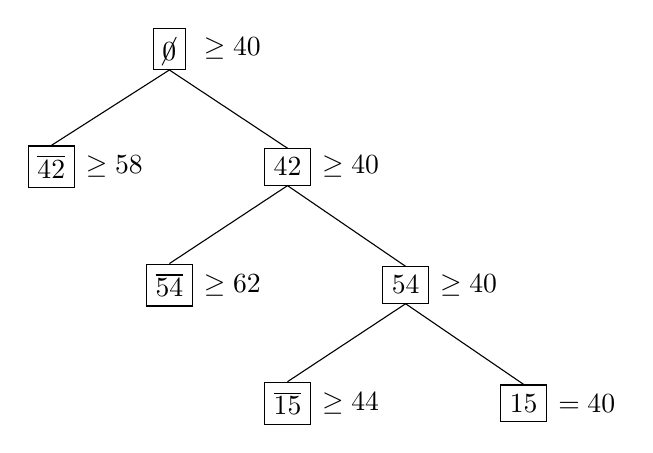
\begin{tikzpicture}[level distance=1.5cm,
  level 1/.style={sibling distance=3cm},
  level 2/.style={sibling distance=3cm}]
  \node [draw] (t1) {$\cancel{0}$}
    child {node (t2) [draw] {$\overline{42}$}}
    child {node (t3) [draw] {$42$}
    child {node (t4) [draw] {$\overline{54}$}}
      child {node (t5) [draw] {$54$}
          child {node (t6) [draw] {$\overline{15}$}}
            child {node (t7) [draw] {$15$}}
      }
    };

    \node (c1) [right of=t1,xshift=-0.2cm]{$\geq{}40$};
    \node (c2) [right of=t2,xshift=-0.2cm]{$\geq{}58$};
    \node (c3) [right of=t3,xshift=-0.2cm]{$\geq{}40$};
    \node (c4) [right of=t4,xshift=-0.2cm]{$\geq{}62$};
    \node (c5) [right of=t5,xshift=-0.2cm]{$\geq{}40$};
    \node (c6) [right of=t6,xshift=-0.2cm]{$\geq{}44$};
    \node (c7) [right of=t7,xshift=-0.2cm]{$=40$};
\end{tikzpicture}
\end{center}
\end{document}
